
\hwpart{I}{Understanding Your Data (10 points)}
Since the goal for generative modeling is to model the distribution of your data, it is important to first understand what does this distribution look like.

The dataset for this course is a custom subset of CelebA, filtered to have specific properties. Your first task is to discover what those properties are.

\question{Visual Exploration}{5}

\subq{a}{2} Visualize a grid of at least 16 random samples from the training set. Include this grid below.

\answerbox{}{
\begin{figure}[H]
    \centering
    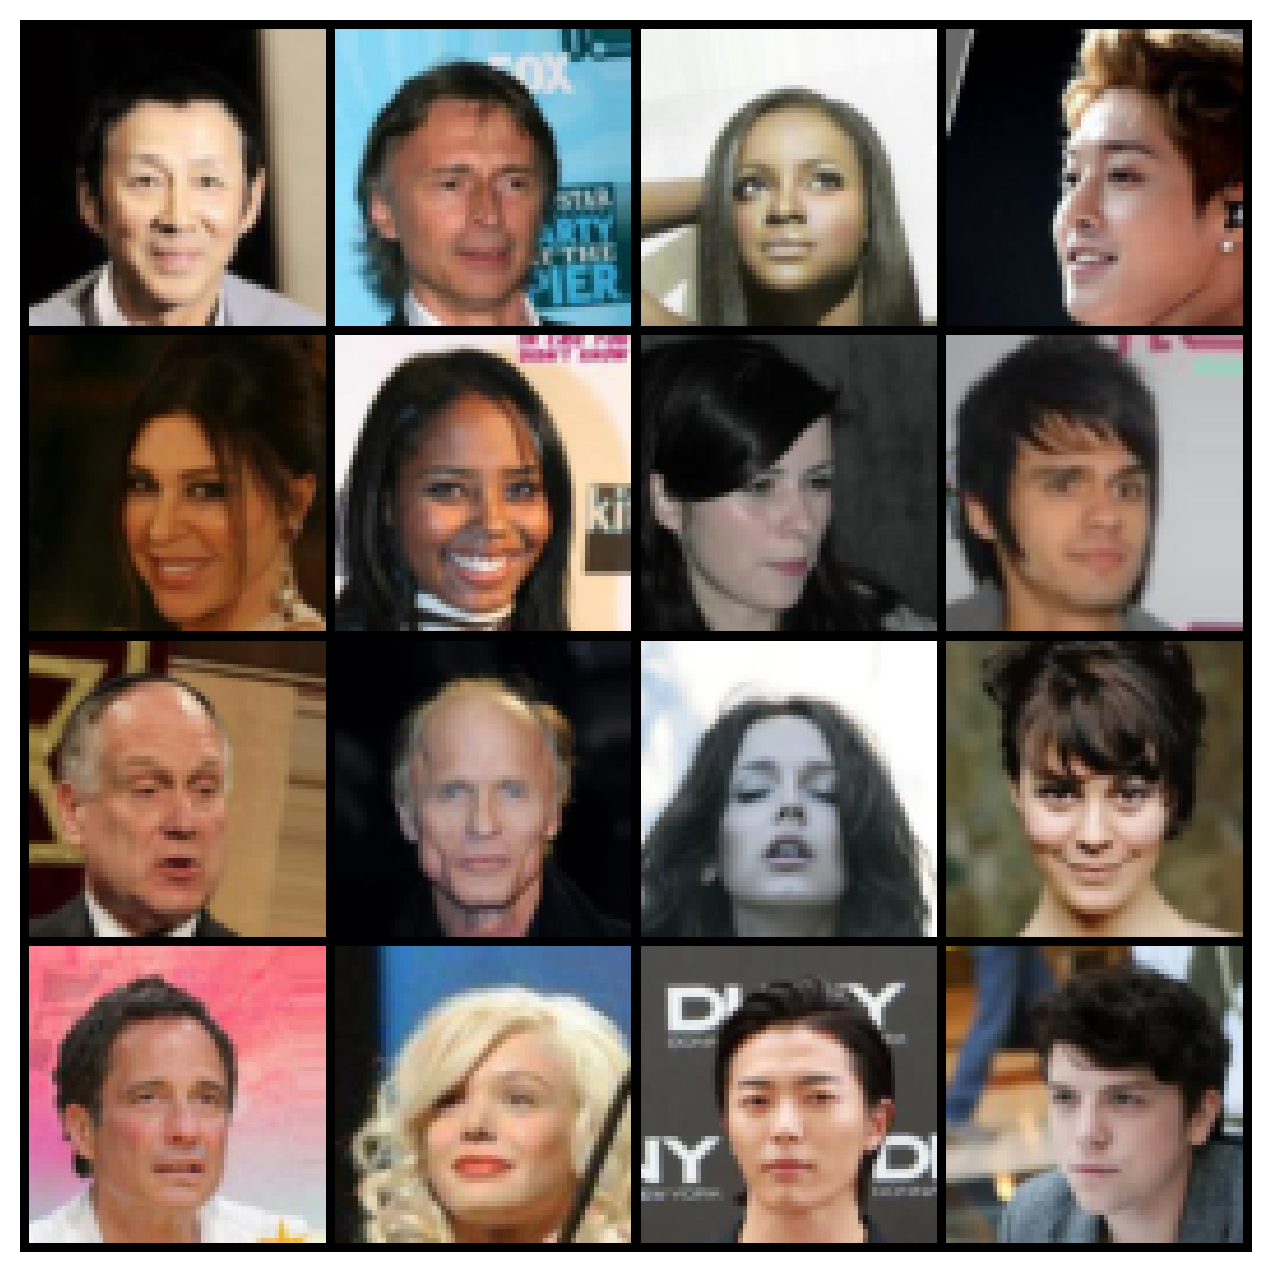
\includegraphics[width=0.65\linewidth]{figures/preview_grid.png}
    \caption{16 random training images ($64\times64$) from the CelebA subset.}
\end{figure}
}
\includeanswer{q1a}

\subq{c}{3} This dataset was filtered from full CelebA using their 40 binary attributes. Based on your visual exploration, hypothesize which attributes were likely used to create this subset. What filtering criteria were used to create this subset? Why?

\answerbox{}{
\textbf{Observation.} In the grid, no face wears glasses or a hat, no man has a beard, nobody has heavy makeup, and every image is sharp. To check this, I computed the fraction of positive labels for each of the 40 attributes in \texttt{attributes.csv} (63{,}715 training images) and compared it with full CelebA (202{,}599 images):

\begin{center}
\small
\begin{tabular}{lrr}
\toprule
Attribute & Full CelebA & Subset \\
\midrule
\texttt{Eyeglasses}       & $\approx 6.5\%$  & $0.0\%$ \\
\texttt{Wearing\_Hat}     & $\approx 4.8\%$  & $0.0\%$ \\
\texttt{Heavy\_Makeup}    & $\approx 38.7\%$ & $0.0\%$ \\
\texttt{Blurry}           & $\approx 5.1\%$  & $0.0\%$ \\
\texttt{No\_Beard}        & $\approx 83.5\%$ & $100.0\%$ \\
\midrule
\texttt{Male}             & $\approx 41.7\%$ & $55.5\%$ \\
\texttt{Wearing\_Lipstick}& $\approx 47.2\%$ & $23.9\%$ \\
\bottomrule
\end{tabular}
\end{center}

\smallskip
Only these five attributes are exactly $0\%$ or $100\%$; every other attribute is strictly between, so it was not used as a filter.

\smallskip
\textbf{Hypothesized filter.}
\[
\texttt{Eyeglasses}=0 \;\wedge\; \texttt{Wearing\_Hat}=0 \;\wedge\; \texttt{Heavy\_Makeup}=0 \;\wedge\; \texttt{Blurry}=0 \;\wedge\; \texttt{No\_Beard}=1 .
\]
\smallskip
The shifts in \texttt{Male} and \texttt{Wearing\_Lipstick} are side effects, not filters: \texttt{Heavy\_Makeup} is labeled almost only on women, so removing it removes more women than removing beards removes men. \texttt{Mustache}, \texttt{Goatee}, and \texttt{Sideburns} are still slightly above zero ($<0.3\%$), which fits a filter on \texttt{No\_Beard} combined with some label noise in CelebA.

\smallskip
\textbf{Why.} These attributes either hide the face (glasses, hats, facial hair), add large appearance variation (heavy makeup), or degrade the image (blur). They form rare modes that are hard to learn with a small model at $64\times64$ resolution, and blurry images would teach the model to generate blur. Removing them (about $31\%$ of CelebA remains) gives a cleaner, more uniform distribution of fully visible faces. This makes the dataset easier to learn on a course compute budget and makes differences in sample quality between methods easier to see.
}
\includeanswer{q1b}

\question{What did you learn?}{5}

\subq{a}{3} Imagine you found a pre-trained diffusion model that can reach SOTA performance on full CelebA (200K diverse faces). Now you generated samples and compared them to this filtered subset using KID or FID. Would you expect the FID and KID score to still be SOTA? Why?
\answerbox{}{
No. FID and KID do not measure image quality on their own. They measure how close the distribution of generated images is to a specific \emph{reference} distribution, by comparing the statistics of Inception features (the mean and covariance for FID, an MMD with a polynomial kernel for KID). A model that is SOTA on full CelebA has learned to match \emph{full} CelebA. It will therefore generate faces with glasses, hats, beards, heavy makeup, and blur in roughly their original proportions, and it will generate more women than the subset contains.

\smallskip
Only about $31\%$ of CelebA passes the filter. A perfect full-CelebA model would therefore produce roughly $69\%$ of samples that break at least one filter rule, i.e.\ samples that have almost no probability under the reference set. This moves the feature mean and widens the covariance relative to the subset, so FID and KID would be clearly worse than SOTA even if every image is photorealistic. ``SOTA'' only holds for the distribution the model was trained on. To be competitive here, the model would need to be fine-tuned on the subset, or its samples would need to be filtered with an attribute classifier (rejection sampling).
}
\includeanswer{q2a}

\subq{b}{2} Based on your exploration, what kind of data augmentation transformation do you plan to use for your training and why?
\answerbox{}{
I use only \textbf{random horizontal flips} ($p=0.5$, \texttt{transforms.RandomHorizontalFlip} in \texttt{src/data/celeba.py}). The faces are aligned, centered, and roughly left-right symmetric. A mirrored face keeps all 40 attributes and is still a valid sample from the same distribution, so flipping effectively doubles the data without changing what the model has to learn.

\smallskip
I avoid other common augmentations. In generative modeling, the model learns the \emph{augmented} distribution and reproduces it in its samples, so an augmentation is only safe if the data distribution does not change under it.
\begin{itemize}[nosep]
    \item \textbf{Random crop, rotation, or scaling:} CelebA faces are aligned with the eyes at fixed positions. These would teach the model to generate shifted or tilted faces.
    \item \textbf{Color jitter:} it changes skin tone and lighting statistics, which pulls the samples away from the reference set and makes FID/KID worse.
    \item \textbf{Vertical flip:} upside-down faces never appear in the data.
    \item \textbf{Blur or noise:} the subset was filtered specifically to remove blurry images.
\end{itemize}
}
\includeanswer{q2b}

% ----------------------------------------------------------------------------
